\section{Линейное и древовидное представление гиперпараметров. Поиск по сетке и случайный поиск.}

\subsection{Представления}

Гиперпараметры можно представлять как список значений для
каждого гиперпараметра (линейный вид).

\begin{figure}[H]
    \centering
    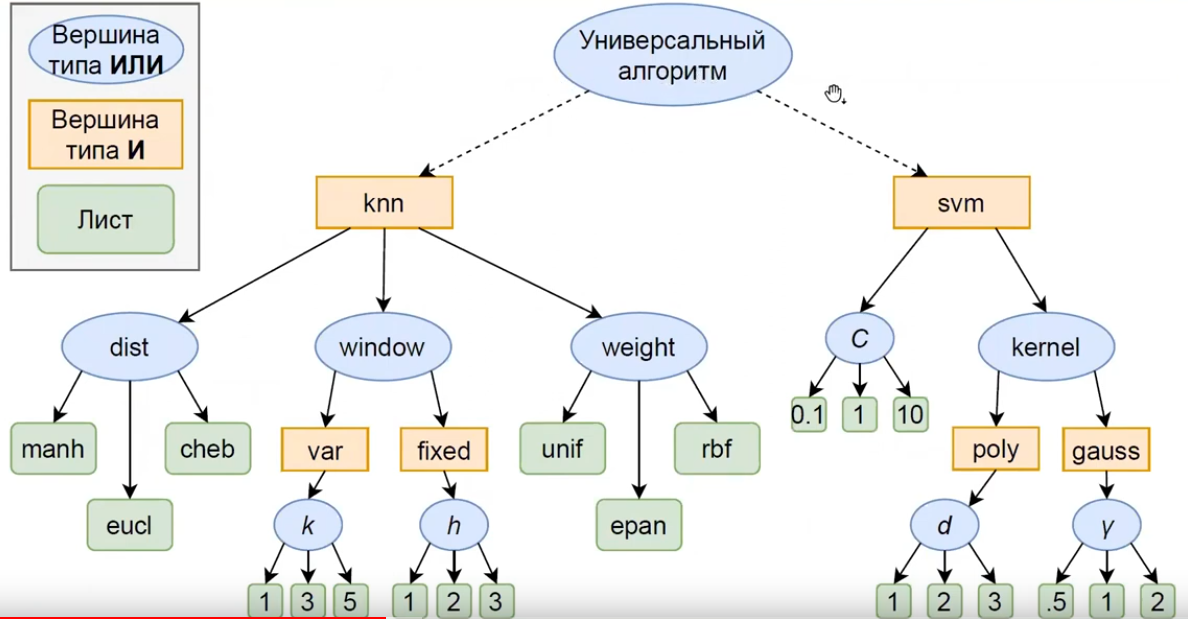
\includegraphics[scale=.4]{images/hp_tree}
    \caption{Древовидное представление}
\end{figure}

В древовидном случае мы строим граф включения для подмножеств
гиперпараметров. (Вершина И значит, что необходимо зайти во все
поддеревья) 

\subsection{Поиск}

\D{
    Поиск по сетке

    \begin{itemize}
        \item Выписываем возможные значения всех гиперпараметров
        \item Дискретизируем числовые параметры
        \item Строим декартово произведение множеств значений
        \item Проходимся по всем комбинациям
    \end{itemize}
}

По сути полный перебор, $k^d$ итераций. Текущий результат зависит
от порядка комбинаций.

Можно посчитать число реальных комбинаций по дереву и не перебирать
независимые ветки.

\D{
    Случайный поиск
    \begin{itemize}
        \item На каждом шаге значения гиперпараметров сэмплируется
        из некоторого распределения
        \item Число итераций ограничивается ручками.
    \end{itemize}
}

Анализ:
\begin{itemize}
    \item Работает с бесконечнозначными гиперпараметрами
    \item Не использует древовидную конфигурацию
    \item Плохо работает с Категориальными гиперпараметрами,
    т.к. может повторять комбинации.
    \item Работает плохо там, где хорош поиск по сетке.
\end{itemize}

Выбор распределения:
\begin{itemize}
    \item Неограниченное: нормальное
    \item С одной границей: экспоненциальное, логнормальное
    \item С двумя: равномерное, бета
\end{itemize}

Можно комбинировать: ищем по сетке, но каждую точку двигаем в
окрестности.

% \begin{figure}[H]
% 	\centering
% 	\begin{minipage}[b]{0.4\textwidth}
% 		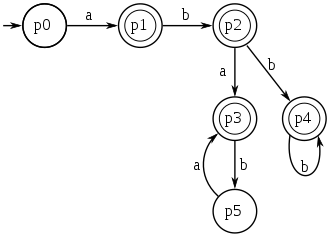
\includegraphics[width=\textwidth]{images/dfa.png}
% 		\caption{Пример графа переходов детерминированного КА.}
% 	\end{minipage}
% 	\hfill
% 	\begin{minipage}[b]{0.4\textwidth}
% 		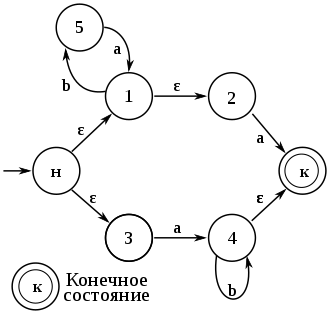
\includegraphics[width=\textwidth]{images/ndfa.png}
% 		\caption{Пример графа переходов недетерминированного КА с самопроизвольными переходами.}
% 	\end{minipage}
% \end{figure}